%% Section 5 — Temporal Dimensions
\section{Temporal Dimensions: Contestation Signals and Regime Response}
\label{sec:temporal}

The first three work packages produce largely synchronic portraits of the datacentering assemblage: how operators narrate themselves, how facilities are rendered visible or invisible, how ownership is constituted through financialisation. Each captures the system's structure at a point in time. The temporal dimension of the CAS, by contrast, concerns dynamics and co-evolution — how the system changes in response to disturbance, and under what structural conditions those changes constitute adaptation rather than absorption. Work Package 4 introduces time. Its purpose is to detect, track, and compare the arc of community contestation against data center development, from the first signs of organised opposition through to whatever regime response, if any, that opposition eventually produces.

\subsection{WP4: Contestation Signals}

The empirical core of WP4 is a multi-source contestation signal corpus assembled from three parallel data streams. News archives — regional and national press accessed via GDELT, NewsAPI, or MediaCloud — provide a longitudinal record of how contestation enters public discourse, how it escalates, and how operators and regulatory actors respond in the textual public sphere. Planning records — council minutes, formal objection filings, environmental impact assessments, moratorium orders — supply the institutional trace of how public signal is translated into regulatory action, with the temporal granularity required to identify discrete transition points. Social media data — principally X/Twitter and Reddit community boards — captures faster-moving, lower-threshold mobilisation that typically precedes or accompanies formal planning processes and provides a signal of contestation intensity that is independent of its institutional reception.

The analytical pipeline applies topic modelling (BERTopic applied to the news and social media corpus) to surface the thematic clusters through which contestation is articulated — energy demand, noise pollution, water consumption, land use conflict, planning law, municipal authority — and tracks how these frames shift as the contestation episode evolves. Event detection algorithms identify discrete inflection points in the longitudinal record: first substantive press coverage, first formal planning objection, moratorium filing, regulatory decision. From these event markers, the pipeline computes the \textit{signal-to-response lag}: the elapsed time between measurable community mobilisation and identifiable regime action, or the absence of any such action at the end of the observation window. This lag variable is the primary comparative output.

The lag variable is WP4's core theoretical contribution to the CAS argument. Complex adaptive systems are characterised not only by their compositional structure — the hierarchies and relationships that WP3 maps — but by the dynamics of adaptation: how the system responds to disturbance signals generated by its components. Community contestation is precisely such a disturbance, and the signal-to-response lag operationalises the key empirical question: under what structural conditions does community feedback produce adaptive regime response? Read alongside WP3's ownership cartography — which establishes how regulatory accountability is distributed or dissolved across ownership tiers — the lag variable becomes a structural diagnostic: it reveals whether a given assemblage configuration is capable of translating local resistance into systemic adjustment, or whether the structural properties of the system (dispersed ownership, legally separated operating and asset-holding entities, fragmented planning authority) insulate it from the disturbances its components generate.

The comparative design makes this concrete. Amsterdam declared a moratorium on new data center construction in 2019, enforced a development halt across the metropolitan region, and lifted the moratorium in 2022 under a differentiated framework requiring stringent energy-efficiency and water-use criteria — a full transition episode with identifiable onset, negotiation, and resolution. Northern Virginia presents the structural contrast: comparable contestation intensity over the same period, no moratorium, and an operator-accommodating state permitting environment that dispersed local accountability rather than consolidating it. The variable that differs is not signal strength but regime structure. The Amsterdam system, as WP3 establishes, had identifiable governance counterparties, concentrated ownership positions capable of entering into binding commitments, and a municipal planning authority with the legal competence to act. The Northern Virginia system, structurally constituted by dispersed REIT ownership, had no equivalent counterparty. WP4 makes this contrast measurable: the same community signal produces different trajectories in the two systems, and the lag variable captures the difference empirically.

As of April 2026, a seed contestation corpus has been constructed from the documented public record — drawing on academic sources \citep{vonderau2019storing}, regional and national press (the \textit{Washington Post}, \textit{Loudoun Now}, \textit{Irish Times}, \textit{The Oregonian}), and official regulatory documents (EirGrid grid capacity reports, Amsterdam Municipality planning decisions, An Bord Pleanála rulings) — across four jurisdictions: Amsterdam, Ashburn/Northern Virginia, Dublin, and The Dalles (Oregon). The corpus documents 58 discrete events between 2007 and 2025, annotated with date, source, and tone valence (\Cref{fig:contestation_signal}). The full live GDELT pull, automated corpus construction, and BERTopic topic modelling are deferred to the server pipeline run; the seed corpus is a methodologically transparent placeholder that establishes the temporal structure of each case and supports the manual cross-case comparison.

The seed corpus supports three first-order observations. First, contestation signal onset differs systematically across jurisdictions: Amsterdam reaches threshold intensity (three or more negative-tone events in a year) in 2019, Dublin in 2020, and Ashburn in 2021. The Dalles, a water-conflict jurisdiction, shows a lower-frequency, episodic contestation pattern with no clear onset year under the threshold measure. Second, negative-tone events constitute the majority of coverage in all jurisdictions (Amsterdam 56\%, Ashburn 59\%, Dublin 81\%, The Dalles 56\%), with Dublin showing the highest sustained negativity — consistent with EirGrid's grid-capacity warnings and An Bord Pleanála's high refusal rate. Third, regime response differs sharply from signal strength: Amsterdam's moratorium (2019) follows signal onset by less than one year; Northern Virginia, with comparable cumulative signal by 2022, produces no moratorium, consistent with the WP3 structural finding that REIT-dominated ownership provides no governance counterparty.

The operationalisation of key constructs — which events constitute signal onset, which count as regime response, how to handle gradual regulatory transitions of the kind Amsterdam's 2022 resolution represents — requires conceptual specification before computation can begin. This is the work package to which the open research community can contribute most immediately: local knowledge about specific contestation episodes, access to municipal planning archives not available through automated collection, and linguistic expertise for non-English jurisdictions are all resources the distributed observatory model is designed to aggregate.

\begin{fullwidth}
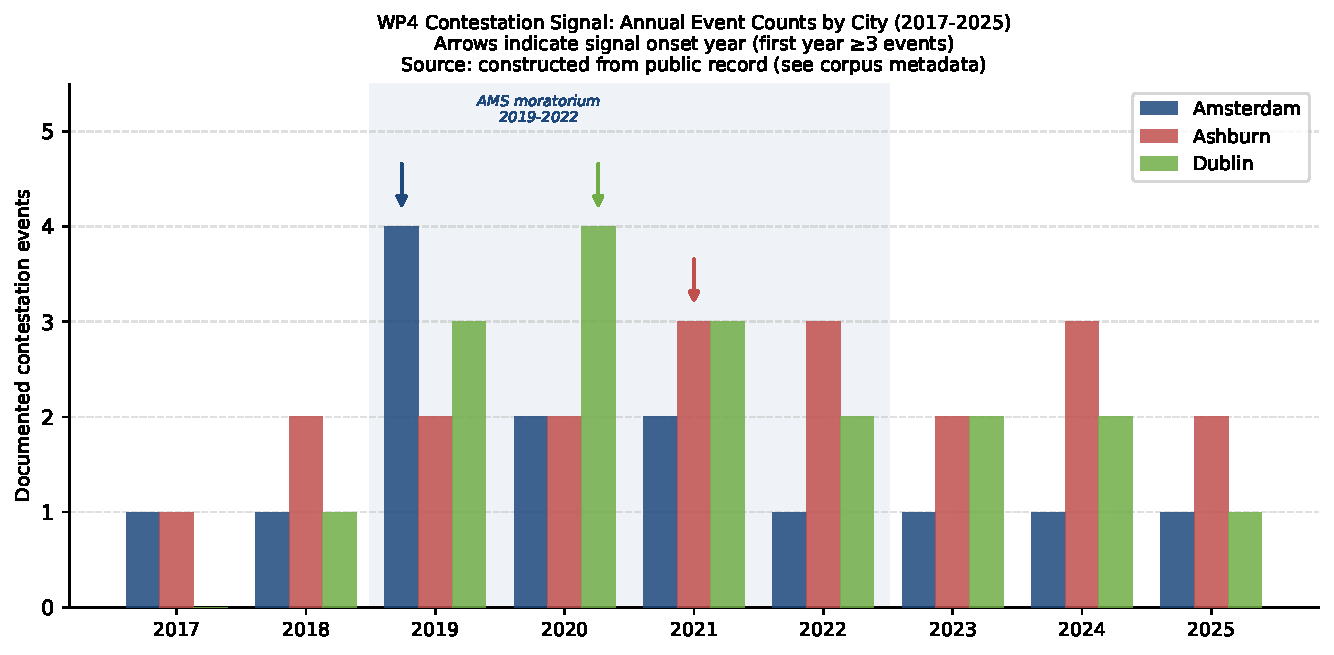
\includegraphics[width=\linewidth]{figures/wp4_contestation_signal}
\vspace{0.4em}
\captionof{figure}{WP4 seed contestation corpus: annual event counts by city (2017--2025), tone-coded. Shaded band: Amsterdam moratorium period (2019--2022). Onset arrows mark the first year reaching the threshold of $\geq 3$ events. Dublin's sustained high negative-tone volume reflects EirGrid grid-capacity constraints and An Bord Pleanála refusals; Northern Virginia's high volume without regime response is the structural contrast case. Data: seed corpus constructed from documented public record (58 events); full GDELT pull deferred to server run.}
\label{fig:contestation_signal}
\end{fullwidth}